
\subsection{The Stack}\label{section:stack}
A \emph{stack} is a data structure to store elements. We can add elements to the stack and take elements from the stack, with the restriction that the element that was added last is always the first element that is taken from the stack. This makes a stack a LIFO (last in, first out) data structure. A stack has two operations:
\begin{itemize}
   \item \textbf{Push}: Add a new element on top of the stack.

   \item \textbf{Pop}: Remove the top (i.e. the most recently added) element from the stack.
\end{itemize}

x86 uses a stack in memory to store the state of function calls, called the \emph{call stack}. Each time a function is called, a \emph{stack frame} is pushed to the call stack. A stack frame stores the arguments, return address, and local variables of a function. When a function returns, the stack frame is popped from the stack.

The call stack grows downwards. When an application starts, the stack pointer is set to some address. When data is pushed on the stack, the stack pointer is \emph{decreased}. Likewise, when data is popped from the stack, the stack pointer is \emph{increased}.

\autoref{fig:stack} illustrates what the stack would look like if a function \texttt{f0} has called another function \texttt{f1}. As we can see, the call frame of the callee is at the top of the stack, on top of the stack frame of the caller.

\begin{figure}[ht]
   \centering
   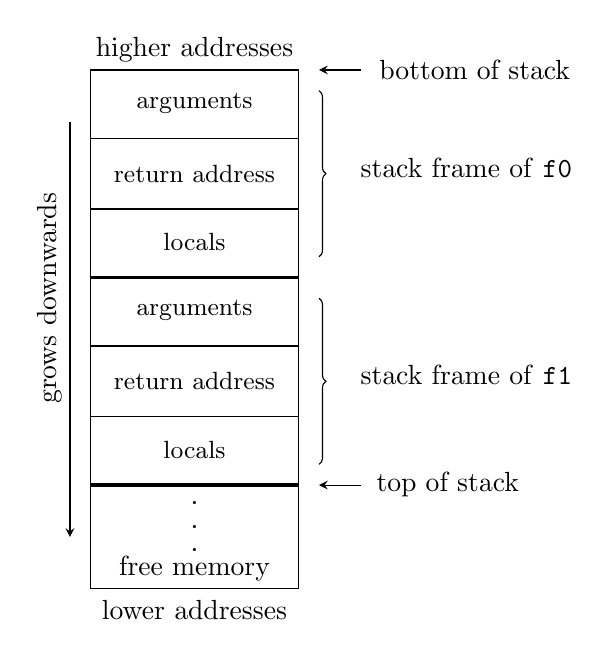
\begin{tikzpicture}[x=0.75pt,y=0.75pt,yscale=-1,xscale=1]

       % Arrow left of stack
       \draw (0,110) node[rotate=90] {grows downwards};
       \draw [-stealth] (10,25) -- (10,225) ;

       % Stack rectangle
       \draw (20,0) -- (120,0) -- (120,250) -- (20,250) -- cycle ;

       % Stack inside
       %% f0
       \draw (70,16) node {\small arguments};
       \draw (20,33) -- (120,33) ;
       \draw (70,50) node {\small return address};
       \draw (20,67) -- (120,67) ;
       \draw (70,83) node {\small locals};

       %% f1
       \draw [very thick] (20,100) -- (120,100) ;
       \draw (70,116) node {\small arguments};
       \draw (20,133) -- (120,133) ;
       \draw (70,150) node {\small return address};
       \draw (20,167) -- (120,167) ;
       \draw (70,183) node {\small locals};

       %% free memory
       \draw [very thick] (20,200) -- (120,200) ;
       \draw (70,220) node[rotate=90] {\large . . . };
       \draw (70,240) node {free memory};

       % Addresses
       \draw (70, -10) node {higher addresses};
       \draw (70, 260) node {lower addresses};

       %% Bottom of stack
       \draw [stealth-] (130,0) -- (150,0) ;
       \draw (205, 0) node {bottom of stack};

       %% Top of stack
       \draw [stealth-] (130,200) -- (150,200) ;
       \draw (192, 200) node {top of stack};

       %% Brace f0
       \draw [decorate, decoration={brace}] (130,10) -- (130,90) ;
       \draw (201,47) node {stack frame of \texttt{f0}};

       %% Brace f1
       \draw [decorate, decoration={brace}] (130,110) -- (130,190) ;
       \draw (201,147) node {stack frame of \texttt{f1}};
   \end{tikzpicture}
   \caption{The layout of the stack when \texttt{f0} has called \texttt{f1}.}
   \label{fig:stack}
\end{figure}

\medskip

Not all data of a program is stored on the stack. Larger and dynamically allocated data is stored in the \emph{heap}. Static and global variables are stored in a separate data segment.
